\PassOptionsToPackage{unicode=true}{hyperref} % options for packages loaded elsewhere
\PassOptionsToPackage{hyphens}{url}
%
\documentclass[]{article}
\usepackage{lmodern}
\usepackage{amssymb,amsmath}
\usepackage{ifxetex,ifluatex}
\usepackage{fixltx2e} % provides \textsubscript
\ifnum 0\ifxetex 1\fi\ifluatex 1\fi=0 % if pdftex
  \usepackage[T1]{fontenc}
  \usepackage[utf8]{inputenc}
  \usepackage{textcomp} % provides euro and other symbols
\else % if luatex or xelatex
  \usepackage{unicode-math}
  \defaultfontfeatures{Ligatures=TeX,Scale=MatchLowercase}
\fi
% use upquote if available, for straight quotes in verbatim environments
\IfFileExists{upquote.sty}{\usepackage{upquote}}{}
% use microtype if available
\IfFileExists{microtype.sty}{%
\usepackage[]{microtype}
\UseMicrotypeSet[protrusion]{basicmath} % disable protrusion for tt fonts
}{}
\IfFileExists{parskip.sty}{%
\usepackage{parskip}
}{% else
\setlength{\parindent}{0pt}
\setlength{\parskip}{6pt plus 2pt minus 1pt}
}
\usepackage{hyperref}
\hypersetup{
            pdfborder={0 0 0},
            breaklinks=true}
\urlstyle{same}  % don't use monospace font for urls
\usepackage[margin=1in]{geometry}
\usepackage{color}
\usepackage{fancyvrb}
\newcommand{\VerbBar}{|}
\newcommand{\VERB}{\Verb[commandchars=\\\{\}]}
\DefineVerbatimEnvironment{Highlighting}{Verbatim}{commandchars=\\\{\}}
% Add ',fontsize=\small' for more characters per line
\usepackage{framed}
\definecolor{shadecolor}{RGB}{248,248,248}
\newenvironment{Shaded}{\begin{snugshade}}{\end{snugshade}}
\newcommand{\AlertTok}[1]{\textcolor[rgb]{0.94,0.16,0.16}{#1}}
\newcommand{\AnnotationTok}[1]{\textcolor[rgb]{0.56,0.35,0.01}{\textbf{\textit{#1}}}}
\newcommand{\AttributeTok}[1]{\textcolor[rgb]{0.77,0.63,0.00}{#1}}
\newcommand{\BaseNTok}[1]{\textcolor[rgb]{0.00,0.00,0.81}{#1}}
\newcommand{\BuiltInTok}[1]{#1}
\newcommand{\CharTok}[1]{\textcolor[rgb]{0.31,0.60,0.02}{#1}}
\newcommand{\CommentTok}[1]{\textcolor[rgb]{0.56,0.35,0.01}{\textit{#1}}}
\newcommand{\CommentVarTok}[1]{\textcolor[rgb]{0.56,0.35,0.01}{\textbf{\textit{#1}}}}
\newcommand{\ConstantTok}[1]{\textcolor[rgb]{0.00,0.00,0.00}{#1}}
\newcommand{\ControlFlowTok}[1]{\textcolor[rgb]{0.13,0.29,0.53}{\textbf{#1}}}
\newcommand{\DataTypeTok}[1]{\textcolor[rgb]{0.13,0.29,0.53}{#1}}
\newcommand{\DecValTok}[1]{\textcolor[rgb]{0.00,0.00,0.81}{#1}}
\newcommand{\DocumentationTok}[1]{\textcolor[rgb]{0.56,0.35,0.01}{\textbf{\textit{#1}}}}
\newcommand{\ErrorTok}[1]{\textcolor[rgb]{0.64,0.00,0.00}{\textbf{#1}}}
\newcommand{\ExtensionTok}[1]{#1}
\newcommand{\FloatTok}[1]{\textcolor[rgb]{0.00,0.00,0.81}{#1}}
\newcommand{\FunctionTok}[1]{\textcolor[rgb]{0.00,0.00,0.00}{#1}}
\newcommand{\ImportTok}[1]{#1}
\newcommand{\InformationTok}[1]{\textcolor[rgb]{0.56,0.35,0.01}{\textbf{\textit{#1}}}}
\newcommand{\KeywordTok}[1]{\textcolor[rgb]{0.13,0.29,0.53}{\textbf{#1}}}
\newcommand{\NormalTok}[1]{#1}
\newcommand{\OperatorTok}[1]{\textcolor[rgb]{0.81,0.36,0.00}{\textbf{#1}}}
\newcommand{\OtherTok}[1]{\textcolor[rgb]{0.56,0.35,0.01}{#1}}
\newcommand{\PreprocessorTok}[1]{\textcolor[rgb]{0.56,0.35,0.01}{\textit{#1}}}
\newcommand{\RegionMarkerTok}[1]{#1}
\newcommand{\SpecialCharTok}[1]{\textcolor[rgb]{0.00,0.00,0.00}{#1}}
\newcommand{\SpecialStringTok}[1]{\textcolor[rgb]{0.31,0.60,0.02}{#1}}
\newcommand{\StringTok}[1]{\textcolor[rgb]{0.31,0.60,0.02}{#1}}
\newcommand{\VariableTok}[1]{\textcolor[rgb]{0.00,0.00,0.00}{#1}}
\newcommand{\VerbatimStringTok}[1]{\textcolor[rgb]{0.31,0.60,0.02}{#1}}
\newcommand{\WarningTok}[1]{\textcolor[rgb]{0.56,0.35,0.01}{\textbf{\textit{#1}}}}
\usepackage{graphicx,grffile}
\makeatletter
\def\maxwidth{\ifdim\Gin@nat@width>\linewidth\linewidth\else\Gin@nat@width\fi}
\def\maxheight{\ifdim\Gin@nat@height>\textheight\textheight\else\Gin@nat@height\fi}
\makeatother
% Scale images if necessary, so that they will not overflow the page
% margins by default, and it is still possible to overwrite the defaults
% using explicit options in \includegraphics[width, height, ...]{}
\setkeys{Gin}{width=\maxwidth,height=\maxheight,keepaspectratio}
\setlength{\emergencystretch}{3em}  % prevent overfull lines
\providecommand{\tightlist}{%
  \setlength{\itemsep}{0pt}\setlength{\parskip}{0pt}}
\setcounter{secnumdepth}{0}
% Redefines (sub)paragraphs to behave more like sections
\ifx\paragraph\undefined\else
\let\oldparagraph\paragraph
\renewcommand{\paragraph}[1]{\oldparagraph{#1}\mbox{}}
\fi
\ifx\subparagraph\undefined\else
\let\oldsubparagraph\subparagraph
\renewcommand{\subparagraph}[1]{\oldsubparagraph{#1}\mbox{}}
\fi

% set default figure placement to htbp
\makeatletter
\def\fps@figure{htbp}
\makeatother


\author{}
\date{\vspace{-2.5em}}

\begin{document}

\begin{Shaded}
\begin{Highlighting}[]
\KeywordTok{library}\NormalTok{(forecast)}
\KeywordTok{library}\NormalTok{(ggplot2)}
\KeywordTok{library}\NormalTok{(tidyr)}
\KeywordTok{library}\NormalTok{(gridExtra)}
\end{Highlighting}
\end{Shaded}

\hypertarget{types-of-noise}{%
\section{Types of noise}\label{types-of-noise}}

\hypertarget{white-noise}{%
\subsection{1.1.1. White noise}\label{white-noise}}

Variable \(w_t\) is a white noise if it meets only three conditions: -
\(E(w_t) = 0\), - \(Var(w_t) = \sigma^2\), - \(cov(w_t, w_s) = 0\).

Note it doesn't have to be normally distributed (then we call it
``gaussian noise'') - but in many cases it is.

\begin{Shaded}
\begin{Highlighting}[]
\KeywordTok{set.seed}\NormalTok{(}\DecValTok{0}\NormalTok{)}
\NormalTok{white_noise =}\StringTok{ }\KeywordTok{rnorm}\NormalTok{(}\DecValTok{200}\NormalTok{)}
\KeywordTok{tsdisplay}\NormalTok{(white_noise, }\DataTypeTok{plot.type =} \StringTok{"histogram"}\NormalTok{, }\DataTypeTok{points =} \OtherTok{FALSE}\NormalTok{)}
\end{Highlighting}
\end{Shaded}

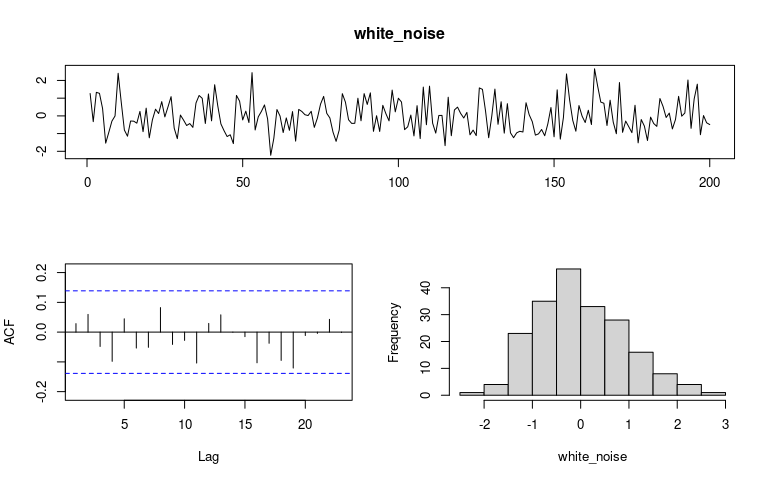
\includegraphics{types_of_noise_files/figure-latex/unnamed-chunk-2-1.pdf}

\begin{Shaded}
\begin{Highlighting}[]
\KeywordTok{mean}\NormalTok{(white_noise)}
\end{Highlighting}
\end{Shaded}

\begin{verbatim}
## [1] -0.01144155
\end{verbatim}

\begin{Shaded}
\begin{Highlighting}[]
\KeywordTok{var}\NormalTok{(white_noise)}
\end{Highlighting}
\end{Shaded}

\begin{verbatim}
## [1] 0.8524895
\end{verbatim}

\begin{Shaded}
\begin{Highlighting}[]
\KeywordTok{set.seed}\NormalTok{(}\DecValTok{0}\NormalTok{) }\CommentTok{# for seed = 7 there is an accidental autocorrelation}
\NormalTok{white_noise2 =}\StringTok{ }\KeywordTok{runif}\NormalTok{(}\DecValTok{200}\NormalTok{, }\DataTypeTok{min =} \DecValTok{-1}\NormalTok{, }\DataTypeTok{max =} \DecValTok{1}\NormalTok{)}
\KeywordTok{tsdisplay}\NormalTok{(white_noise2, }\DataTypeTok{plot.type =} \StringTok{"histogram"}\NormalTok{, }\DataTypeTok{points =} \OtherTok{FALSE}\NormalTok{)}
\end{Highlighting}
\end{Shaded}

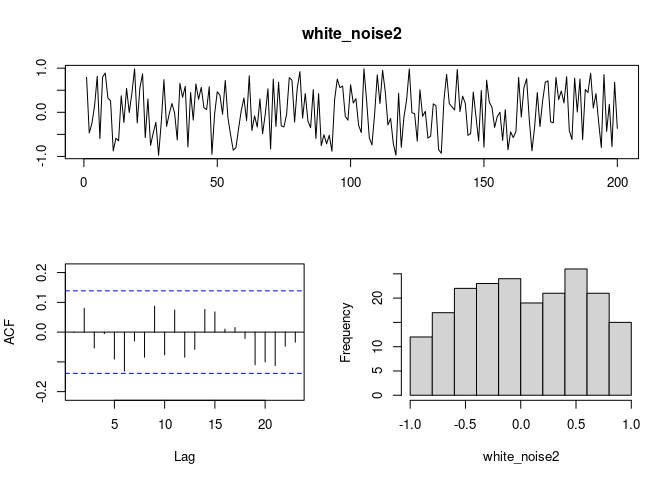
\includegraphics{types_of_noise_files/figure-latex/unnamed-chunk-4-1.pdf}

\begin{Shaded}
\begin{Highlighting}[]
\KeywordTok{mean}\NormalTok{(white_noise2)}
\end{Highlighting}
\end{Shaded}

\begin{verbatim}
## [1] 0.03645731
\end{verbatim}

\begin{Shaded}
\begin{Highlighting}[]
\KeywordTok{var}\NormalTok{(white_noise2) }\CommentTok{# 1/3 is a theoretical value}
\end{Highlighting}
\end{Shaded}

\begin{verbatim}
## [1] 0.2909825
\end{verbatim}

\hypertarget{autoreggresive-processes-arp}{%
\subsection{Autoreggresive Processes
AR(p)}\label{autoreggresive-processes-arp}}

The Autoregressive process is given by the equation

\[X_t = \sum^p_{i=1} \theta_i X_{t-i} + w_t.\]

\hypertarget{ar1}{%
\subsubsection{AR(1)}\label{ar1}}

AR(1) process \[X_t = \theta X_{t-1} + w_t\]

is stationary if \(|\theta| < 1\). In R we can simulate such process
using \texttt{arima.sim} function. Greater absolute value results in
greater ``amplitude'' and negative theta causes oscilations from
positive to negative.

\begin{Shaded}
\begin{Highlighting}[]
\NormalTok{N <-}\StringTok{ }\DecValTok{200}
\NormalTok{ar1_processes <-}\StringTok{ }\KeywordTok{matrix}\NormalTok{(}\DataTypeTok{nrow =} \DecValTok{7}\NormalTok{, }\DataTypeTok{ncol =}\NormalTok{ N)}
\NormalTok{ar1_processes[}\DecValTok{1}\NormalTok{,] <-}\StringTok{ }\DecValTok{1}\OperatorTok{:}\NormalTok{N}
\NormalTok{ar1_processes[}\DecValTok{2}\NormalTok{,] <-}\StringTok{ }\KeywordTok{arima.sim}\NormalTok{(}\DataTypeTok{model =} \KeywordTok{list}\NormalTok{(}\DataTypeTok{ar =} \KeywordTok{c}\NormalTok{(}\FloatTok{0.1}\NormalTok{)), }\DataTypeTok{n =}\NormalTok{ N)}
\NormalTok{ar1_processes[}\DecValTok{3}\NormalTok{,] <-}\StringTok{ }\KeywordTok{arima.sim}\NormalTok{(}\DataTypeTok{model =} \KeywordTok{list}\NormalTok{(}\DataTypeTok{ar =} \KeywordTok{c}\NormalTok{(}\FloatTok{0.5}\NormalTok{)), }\DataTypeTok{n =}\NormalTok{ N)}
\NormalTok{ar1_processes[}\DecValTok{4}\NormalTok{,] <-}\StringTok{ }\KeywordTok{arima.sim}\NormalTok{(}\DataTypeTok{model =} \KeywordTok{list}\NormalTok{(}\DataTypeTok{ar =} \KeywordTok{c}\NormalTok{(}\FloatTok{0.9}\NormalTok{)), }\DataTypeTok{n =}\NormalTok{ N)}
\NormalTok{ar1_processes[}\DecValTok{5}\NormalTok{,] <-}\StringTok{ }\KeywordTok{arima.sim}\NormalTok{(}\DataTypeTok{model =} \KeywordTok{list}\NormalTok{(}\DataTypeTok{ar =} \KeywordTok{c}\NormalTok{(}\OperatorTok{-}\FloatTok{0.1}\NormalTok{)), }\DataTypeTok{n =}\NormalTok{ N)}
\NormalTok{ar1_processes[}\DecValTok{6}\NormalTok{,] <-}\StringTok{ }\KeywordTok{arima.sim}\NormalTok{(}\DataTypeTok{model =} \KeywordTok{list}\NormalTok{(}\DataTypeTok{ar =} \KeywordTok{c}\NormalTok{(}\OperatorTok{-}\FloatTok{0.5}\NormalTok{)), }\DataTypeTok{n =}\NormalTok{ N)}
\NormalTok{ar1_processes[}\DecValTok{7}\NormalTok{,] <-}\StringTok{ }\KeywordTok{arima.sim}\NormalTok{(}\DataTypeTok{model =} \KeywordTok{list}\NormalTok{(}\DataTypeTok{ar =} \KeywordTok{c}\NormalTok{(}\OperatorTok{-}\FloatTok{0.9}\NormalTok{)), }\DataTypeTok{n =}\NormalTok{ N)}

\CommentTok{# Note: you can use arima.sim only to simulate a stationary process. To simulate non-stationary one,}
\CommentTok{# use Arima.}

\NormalTok{ar1_processes <-}\StringTok{ }\KeywordTok{as.data.frame}\NormalTok{(}\KeywordTok{t}\NormalTok{(ar1_processes)) }
\KeywordTok{colnames}\NormalTok{(ar1_processes) <-}\StringTok{ }\KeywordTok{c}\NormalTok{(}
  \StringTok{"time"}\NormalTok{, }\StringTok{"theta_0.1"}\NormalTok{, }\StringTok{"theta_0.5"}\NormalTok{, }\StringTok{"theta_0.9"}\NormalTok{, }\StringTok{"theta_-0.1"}\NormalTok{, }\StringTok{"theta_-0.5"}\NormalTok{, }\StringTok{"theta_-0.9"}\NormalTok{)}

\NormalTok{ar1_processes }\OperatorTok\StringTok{ }\KeywordTok{pivot_longer}\NormalTok{(}\DataTypeTok{cols =} \DecValTok{2}\OperatorTok{:}\DecValTok{7}\NormalTok{) }\OperatorTok\StringTok{ }
\StringTok{  }\KeywordTok{ggplot}\NormalTok{(}\KeywordTok{aes}\NormalTok{(}\DataTypeTok{x =}\NormalTok{ time, }\DataTypeTok{y =}\NormalTok{ value, }\DataTypeTok{col =}\NormalTok{ name)) }\OperatorTok{+}
\StringTok{  }\KeywordTok{geom_line}\NormalTok{() }\OperatorTok{+}\StringTok{ }
\StringTok{  }\KeywordTok{ggtitle}\NormalTok{(}\StringTok{"AR(1) processes with different coefficient (only stationary, i.e. |theta| < 1 allowed by arima.sim)"}\NormalTok{) }\OperatorTok{+}
\StringTok{  }\KeywordTok{theme}\NormalTok{(}\DataTypeTok{legend.position =} \StringTok{"bottom"}\NormalTok{)}
\end{Highlighting}
\end{Shaded}

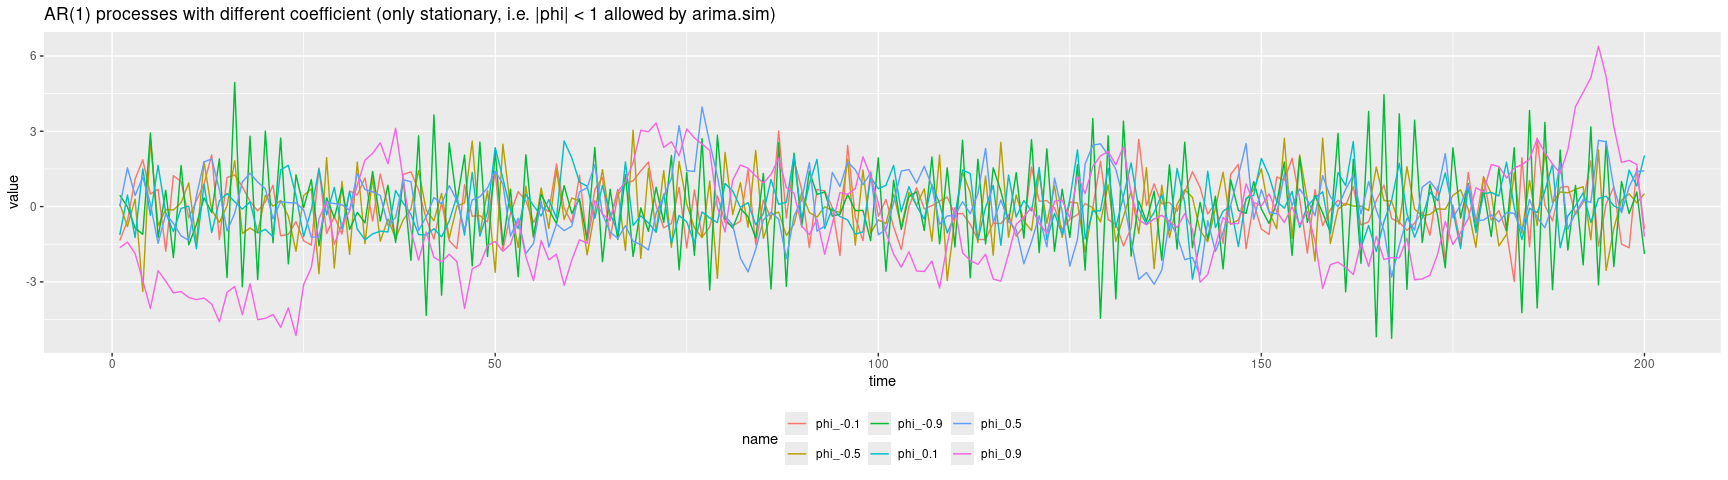
\includegraphics{types_of_noise_files/figure-latex/unnamed-chunk-6-1.pdf}

\begin{Shaded}
\begin{Highlighting}[]
\NormalTok{ar1_acfs <-}\StringTok{ }\KeywordTok{list}\NormalTok{()}
\ControlFlowTok{for}\NormalTok{ (name }\ControlFlowTok{in} \KeywordTok{colnames}\NormalTok{(ar1_processes)[}\OperatorTok{-}\DecValTok{1}\NormalTok{])\{}
\NormalTok{  ar1_acfs[[name]] <-}\StringTok{ }\NormalTok{ar1_processes[name] }\OperatorTok\StringTok{ }\KeywordTok{ggAcf}\NormalTok{() }\OperatorTok{+}
\StringTok{    }\KeywordTok{ggtitle}\NormalTok{(}\KeywordTok{paste}\NormalTok{(}\StringTok{"AR(1) with"}\NormalTok{, name))}
\NormalTok{\}}

\NormalTok{gridExtra}\OperatorTok{::}\KeywordTok{grid.arrange}\NormalTok{(}
  \DataTypeTok{grobs =}\NormalTok{ ar1_acfs, }\DataTypeTok{nrow =} \DecValTok{2}\NormalTok{, }\DataTypeTok{top =} \StringTok{"ACF plots for AR(1) process with different theta"}\NormalTok{)}
\end{Highlighting}
\end{Shaded}

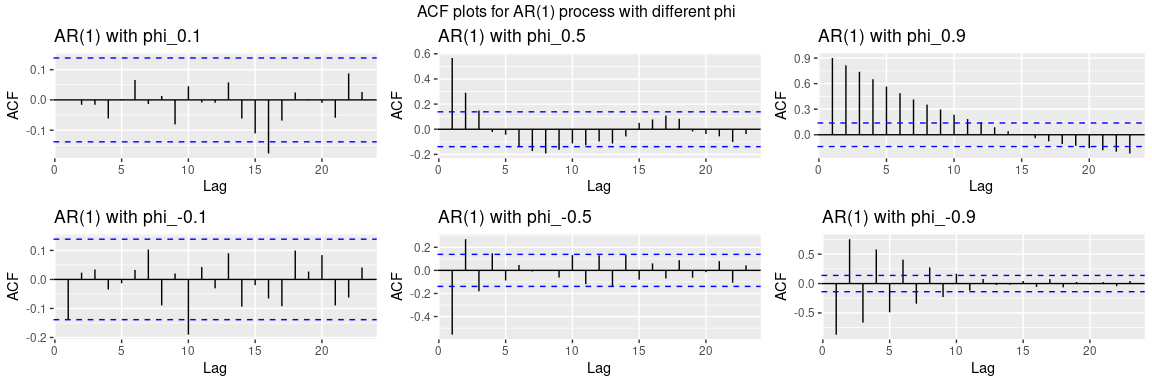
\includegraphics{types_of_noise_files/figure-latex/unnamed-chunk-7-1.pdf}

\begin{Shaded}
\begin{Highlighting}[]
\NormalTok{ar1_pacfs <-}\StringTok{ }\KeywordTok{list}\NormalTok{()}
\ControlFlowTok{for}\NormalTok{ (name }\ControlFlowTok{in} \KeywordTok{colnames}\NormalTok{(ar1_processes)[}\OperatorTok{-}\DecValTok{1}\NormalTok{])\{}
\NormalTok{  ar1_pacfs[[name]] <-}\StringTok{ }\NormalTok{ar1_processes[name] }\OperatorTok\StringTok{ }\KeywordTok{ggPacf}\NormalTok{() }\OperatorTok{+}
\StringTok{    }\KeywordTok{ggtitle}\NormalTok{(}\KeywordTok{paste}\NormalTok{(}\StringTok{"AR(1) with"}\NormalTok{, name))}
\NormalTok{\}}

\NormalTok{gridExtra}\OperatorTok{::}\KeywordTok{grid.arrange}\NormalTok{(}
  \DataTypeTok{grobs =}\NormalTok{ ar1_pacfs, }\DataTypeTok{nrow =} \DecValTok{2}\NormalTok{, }\DataTypeTok{top =} \StringTok{"PACF plots for AR(1) process with different theta"}\NormalTok{)}
\end{Highlighting}
\end{Shaded}

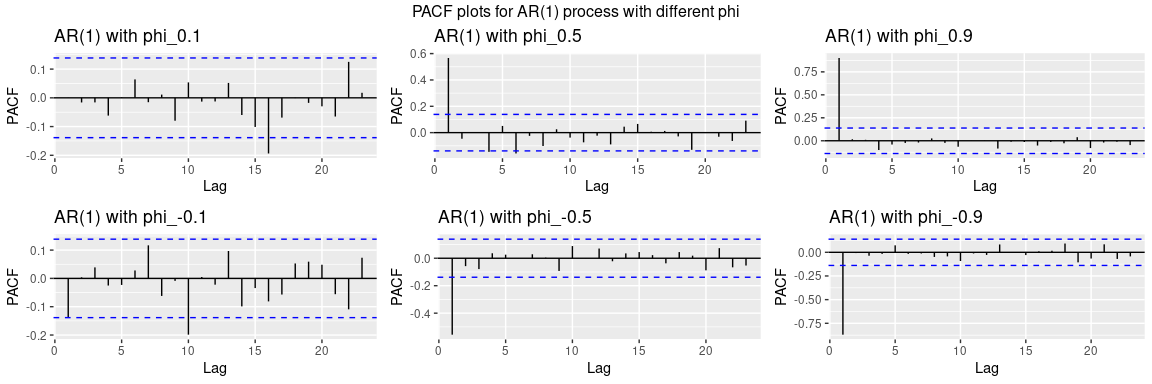
\includegraphics{types_of_noise_files/figure-latex/unnamed-chunk-8-1.pdf}

\end{document}
